% ============================================================
\chapter{Apprentissage non supervis\'e~--- Clustering}
\label{ch:non-supervise}
\index{apprentissage!non supervis\'e}\index{clustering}
% ============================================================

\section{Introduction}

En apprentissage non supervis\'e, on dispose d'un jeu de donn\'ees
$\mathcal{D} = \{\bm{x}_1, \ldots, \bm{x}_n\}$ avec $\bm{x}_i \in \R^d$,
\emph{sans \'etiquettes}. L'objectif du \textbf{clustering} (partitionnement)
est de regrouper les observations en $K$ groupes
$\mathcal{C} = \{C_1, \ldots, C_K\}$ tels que les points d'un m\^eme cluster
soient <<~similaires~>> et ceux de clusters diff\'erents soient <<~dissemblables~>>.

\begin{definition}[Partition]
Une \textbf{partition} de $\mathcal{D}$ en $K$ clusters est une famille
$\{C_1, \ldots, C_K\}$ telle que~:
\begin{enumerate}
  \item $C_k \neq \emptyset$ pour tout $k$,
  \item $C_i \cap C_j = \emptyset$ pour $i \neq j$,
  \item $\bigcup_{k=1}^K C_k = \mathcal{D}$.
\end{enumerate}
\end{definition}

% ============================================================
\section{$k$-Means}
\label{sec:kmeans}
\index{k-Means}
% ============================================================

\subsection{Formulation}

\begin{definition}[$k$-Means]
L'algorithme $k$-Means cherche une partition $\{C_1, \ldots, C_K\}$ et des
centro\"ides $\{\bm{\mu}_1, \ldots, \bm{\mu}_K\}$ minimisant l'\textbf{inertie
intra-cluster}~:
\begin{equation}
  J(\mathcal{C}, \bm{\mu}) = \sum_{k=1}^K \sum_{\bm{x}_i \in C_k}
  \norm{\bm{x}_i - \bm{\mu}_k}^2
  \label{eq:kmeans-obj}
\end{equation}
\end{definition}

Ce probl\`eme est NP-difficile en g\'en\'eral. L'algorithme de Lloyd fournit
une heuristique efficace.

\subsection{Algorithme de Lloyd}

\begin{algorithme}[title=\textbf{$k$-Means (Lloyd)}]
\textbf{Entr\'ee~:} $\mathcal{D} = \{\bm{x}_1, \ldots, \bm{x}_n\}$, nombre
de clusters $K$.

\begin{enumerate}
  \item \textbf{Initialisation~:} choisir $K$ centro\"ides initiaux
    $\bm{\mu}_1^{(0)}, \ldots, \bm{\mu}_K^{(0)}$.
  \item \textbf{R\'ep\'eter} jusqu'\`a convergence~:
    \begin{enumerate}
      \item \textbf{Assignation~:} pour chaque $\bm{x}_i$, affecter au cluster
        le plus proche~:
        \begin{equation}
          c_i^{(t)} = \argmin_{k \in \{1, \ldots, K\}} \norm{\bm{x}_i - \bm{\mu}_k^{(t)}}^2
        \end{equation}
      \item \textbf{Mise \`a jour~:} recalculer les centro\"ides~:
        \begin{equation}
          \bm{\mu}_k^{(t+1)} = \frac{1}{|C_k^{(t)}|} \sum_{\bm{x}_i \in C_k^{(t)}} \bm{x}_i
        \end{equation}
    \end{enumerate}
\end{enumerate}
\textbf{Sortie~:} partition $\{C_1, \ldots, C_K\}$ et centro\"ides
$\{\bm{\mu}_1, \ldots, \bm{\mu}_K\}$.
\end{algorithme}

\begin{center}
\begin{tikzpicture}[scale=0.85]
  % Iteration 0
  \begin{scope}[shift={(0,0)}]
    \node[font=\small\bfseries] at (2,3.8) {$t=0$ (init)};
    \foreach \x/\y in {0.5/1.0, 1.0/1.5, 0.8/0.6, 1.5/1.2,
                        3.0/2.5, 3.5/3.0, 2.8/2.8, 3.2/2.2} {
      \fill[gray] (\x,\y) circle (2pt);
    }
    \fill[red,draw=black] (1.0,2.5) circle (4pt);
    \fill[blue,draw=black] (3.0,1.0) circle (4pt);
  \end{scope}
  % Iteration 1
  \begin{scope}[shift={(5.5,0)}]
    \node[font=\small\bfseries] at (2,3.8) {$t=1$ (assign)};
    \foreach \x/\y in {0.5/1.0, 1.0/1.5, 0.8/0.6, 1.5/1.2} {
      \fill[red!60] (\x,\y) circle (2pt);
    }
    \foreach \x/\y in {3.0/2.5, 3.5/3.0, 2.8/2.8, 3.2/2.2} {
      \fill[blue!60] (\x,\y) circle (2pt);
    }
    \fill[red,draw=black] (0.95,1.075) circle (4pt);
    \fill[blue,draw=black] (3.125,2.625) circle (4pt);
  \end{scope}
  % Iteration 2
  \begin{scope}[shift={(11,0)}]
    \node[font=\small\bfseries] at (2,3.8) {$t=2$ (converge)};
    \foreach \x/\y in {0.5/1.0, 1.0/1.5, 0.8/0.6, 1.5/1.2} {
      \fill[red!60] (\x,\y) circle (2pt);
    }
    \foreach \x/\y in {3.0/2.5, 3.5/3.0, 2.8/2.8, 3.2/2.2} {
      \fill[blue!60] (\x,\y) circle (2pt);
    }
    \fill[red,draw=black] (0.95,1.075) circle (4pt);
    \fill[blue,draw=black] (3.125,2.625) circle (4pt);
    \node[font=\scriptsize,green!50!black] at (2,0) {\checkmark~Convergence};
  \end{scope}
  \draw[-{Stealth},thick] (4.2,1.8) -- (5.0,1.8);
  \draw[-{Stealth},thick] (9.7,1.8) -- (10.5,1.8);
\end{tikzpicture}
\end{center}

\subsection{Convergence}

\begin{theoreme}[Convergence de $k$-Means]
L'algorithme de Lloyd converge en un nombre fini d'it\'erations.
\end{theoreme}

\begin{proof}[Esquisse de preuve]
\`A chaque it\'eration, l'\'etape d'assignation et l'\'etape de mise \`a jour
diminuent (ou laissent inchang\'ee) la fonction objectif $J$.
\begin{itemize}
  \item \textbf{Assignation~:} \`a $\bm{\mu}$ fix\'e, assigner chaque point
    au centro\"ide le plus proche minimise $J$.
  \item \textbf{Mise \`a jour~:} \`a $\mathcal{C}$ fix\'e, le minimum de
    $\sum_{\bm{x}_i \in C_k} \norm{\bm{x}_i - \bm{\mu}_k}^2$ par rapport \`a
    $\bm{\mu}_k$ est atteint en $\bm{\mu}_k = \frac{1}{|C_k|}\sum_{\bm{x}_i
    \in C_k} \bm{x}_i$ (d\'eriv\'ee nulle).
\end{itemize}
Comme $J \geq 0$ est d\'ecroissante et que le nombre de partitions est fini
($\leq K^n$), l'algorithme converge. N\'eanmoins, il converge vers un
\emph{minimum local}, pas n\'ecessairement global.
\end{proof}

\subsection{Initialisation~: $k$-Means++}
\index{k-Means++}

\begin{attention}[title=\textbf{Sensibilit\'e \`a l'initialisation}]
L'algorithme de Lloyd est tr\`es sensible au choix initial des centro\"ides.
Une mauvaise initialisation peut conduire \`a un minimum local de mauvaise
qualit\'e. La strat\'egie \textbf{$k$-Means++} att\'enue ce probl\`eme.
\end{attention}

\begin{algorithme}[title=\textbf{Initialisation $k$-Means++}]
\begin{enumerate}
  \item Choisir $\bm{\mu}_1$ uniform\'ement au hasard parmi les donn\'ees.
  \item Pour $k = 2, \ldots, K$~:
    \begin{enumerate}
      \item Pour chaque $\bm{x}_i$, calculer $d_i = \min_{j < k}
        \norm{\bm{x}_i - \bm{\mu}_j}^2$.
      \item Choisir $\bm{\mu}_k = \bm{x}_i$ avec probabilit\'e
        $\frac{d_i}{\sum_j d_j}$.
    \end{enumerate}
  \item Lancer l'algorithme de Lloyd avec ces centro\"ides.
\end{enumerate}
\end{algorithme}

\begin{theoreme}[Garantie $k$-Means++ {\cite{arthur2007}}]
L'initialisation $k$-Means++ garantit que l'inertie attendue satisfait~:
\begin{equation}
  \E[J] \leq 8(\ln K + 2) \cdot J_{\text{opt}}
\end{equation}
o\`u $J_{\text{opt}}$ est l'inertie optimale.
\end{theoreme}

% ============================================================
\section{Mod\`eles de m\'elange gaussien (GMM)}
\label{sec:gmm}
\index{GMM}\index{m\'elange gaussien}
% ============================================================

\subsection{Mod\`ele}

\begin{definition}[M\'elange de gaussiennes]
Un \textbf{mod\`ele de m\'elange gaussien} \`a $K$ composantes suppose que
chaque observation est g\'en\'er\'ee par~:
\begin{equation}
  p(\bm{x}) = \sum_{k=1}^K \pi_k \, \mathcal{N}(\bm{x} \mid \bm{\mu}_k,
  \bm{\Sigma}_k)
  \label{eq:gmm}
\end{equation}
o\`u $\pi_k \geq 0$ sont les poids de m\'elange ($\sum_k \pi_k = 1$),
$\bm{\mu}_k$ les moyennes, et $\bm{\Sigma}_k$ les matrices de covariance.
\end{definition}

On introduit une variable latente $z_i \in \{1, \ldots, K\}$ indiquant la
composante de chaque observation. Alors~:
\begin{equation}
  p(z_i = k) = \pi_k, \qquad p(\bm{x}_i \mid z_i = k) =
  \mathcal{N}(\bm{x}_i \mid \bm{\mu}_k, \bm{\Sigma}_k)
\end{equation}

\subsection{Algorithme EM}
\index{algorithme EM}

La log-vraisemblance du m\'elange est~:
\begin{equation}
  \ell(\bm{\theta}) = \sum_{i=1}^n \ln \left( \sum_{k=1}^K \pi_k \,
  \mathcal{N}(\bm{x}_i \mid \bm{\mu}_k, \bm{\Sigma}_k) \right)
\end{equation}
La pr\'esence du logarithme d'une somme rend l'optimisation directe difficile.
L'algorithme \textbf{Esp\'erance-Maximisation (EM)} r\'esout ce probl\`eme de
mani\`ere it\'erative.

\begin{formules}[title=\textbf{Algorithme EM pour GMM}]
\textbf{E-step~:} calculer les responsabilit\'es~:
\begin{equation}
  \gamma_{ik} = p(z_i = k \mid \bm{x}_i, \bm{\theta}^{(t)}) =
  \frac{\pi_k^{(t)} \, \mathcal{N}(\bm{x}_i \mid \bm{\mu}_k^{(t)},
  \bm{\Sigma}_k^{(t)})}{\sum_{j=1}^K \pi_j^{(t)} \,
  \mathcal{N}(\bm{x}_i \mid \bm{\mu}_j^{(t)}, \bm{\Sigma}_j^{(t)})}
  \label{eq:e-step}
\end{equation}

\textbf{M-step~:} mettre \`a jour les param\`etres. Soit $N_k = \sum_{i=1}^n
\gamma_{ik}$~:
\begin{align}
  \bm{\mu}_k^{(t+1)} &= \frac{1}{N_k} \sum_{i=1}^n \gamma_{ik}\, \bm{x}_i
  \label{eq:m-step-mu} \\
  \bm{\Sigma}_k^{(t+1)} &= \frac{1}{N_k} \sum_{i=1}^n \gamma_{ik}\,
  (\bm{x}_i - \bm{\mu}_k^{(t+1)})(\bm{x}_i - \bm{\mu}_k^{(t+1)})^\top
  \label{eq:m-step-sigma} \\
  \pi_k^{(t+1)} &= \frac{N_k}{n}
  \label{eq:m-step-pi}
\end{align}
\end{formules}

\begin{theoreme}[Monotonie de EM]
L'algorithme EM garantit que la log-vraisemblance est non d\'ecroissante~:
\begin{equation}
  \ell(\bm{\theta}^{(t+1)}) \geq \ell(\bm{\theta}^{(t)})
\end{equation}
La preuve repose sur l'in\'egalit\'e de Jensen et la construction de la borne
inf\'erieure (ELBO).
\end{theoreme}

\begin{intuition}[title=\textbf{EM vs $k$-Means}]
\begin{itemize}
  \item $k$-Means est un cas particulier de EM o\`u toutes les covariances sont
    $\sigma^2 \bm{I}$ et les responsabilit\'es sont <<~dures~>> ($\gamma_{ik}
    \in \{0,1\}$).
  \item EM effectue une assignation <<~souple~>> (\emph{soft clustering}).
  \item EM mod\'elise des clusters elliptiques, pas seulement sph\'eriques.
\end{itemize}
\end{intuition}

\begin{center}
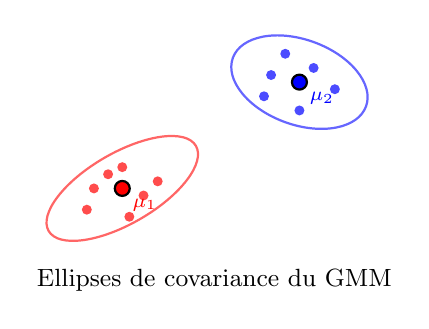
\begin{tikzpicture}[scale=0.9]
  % Cluster 1
  \draw[red!60, thick, rotate around={30:(1.5,1.5)}]
    (1.5,1.5) ellipse (1.2cm and 0.5cm);
  \foreach \x/\y in {1.0/1.2, 1.3/1.7, 1.8/1.4, 1.5/1.8, 1.1/1.5,
                      2.0/1.6, 1.6/1.1} {
    \fill[red!70] (\x,\y) circle (2pt);
  }
  \fill[red,draw=black,thick] (1.5,1.5) circle (3pt)
    node[below right,font=\scriptsize] {$\bm{\mu}_1$};
  % Cluster 2
  \draw[blue!60, thick, rotate around={-20:(4.0,3.0)}]
    (4.0,3.0) ellipse (1.0cm and 0.6cm);
  \foreach \x/\y in {3.5/2.8, 4.2/3.2, 3.8/3.4, 4.5/2.9, 4.0/2.6,
                      3.6/3.1} {
    \fill[blue!70] (\x,\y) circle (2pt);
  }
  \fill[blue,draw=black,thick] (4.0,3.0) circle (3pt)
    node[below right,font=\scriptsize] {$\bm{\mu}_2$};
  \node[font=\small] at (2.8,0.2) {Ellipses de covariance du GMM};
\end{tikzpicture}
\end{center}

% ============================================================
\section{DBSCAN}
\label{sec:dbscan}
\index{DBSCAN}
% ============================================================

\begin{definition}[DBSCAN]
\textbf{DBSCAN} (\emph{Density-Based Spatial Clustering of Applications with
Noise}) est un algorithme fond\'e sur la densit\'e, param\'etr\'e par~:
\begin{itemize}
  \item $\varepsilon > 0$~: rayon du voisinage,
  \item \texttt{min\_samples}~: nombre minimum de points dans le
    $\varepsilon$-voisinage pour qu'un point soit <<~core~>>.
\end{itemize}
\end{definition}

\begin{definition}[$\varepsilon$-voisinage]
Le $\varepsilon$-voisinage d'un point $\bm{x}$ est~:
\begin{equation}
  N_\varepsilon(\bm{x}) = \{\bm{x}' \in \mathcal{D} : \norm{\bm{x} - \bm{x}'}
  \leq \varepsilon\}
\end{equation}
\end{definition}

\begin{definition}[Types de points]
\begin{itemize}
  \item \textbf{Point noyau} (\emph{core point})~:
    $|N_\varepsilon(\bm{x})| \geq \texttt{min\_samples}$.
  \item \textbf{Point fronti\`ere} (\emph{border point})~: non noyau mais dans
    le $\varepsilon$-voisinage d'un point noyau.
  \item \textbf{Point bruit} (\emph{noise})~: ni noyau, ni fronti\`ere.
\end{itemize}
\end{definition}

\begin{algorithme}[title=\textbf{DBSCAN}]
\begin{enumerate}
  \item Marquer tous les points comme <<~non visit\'es~>>.
  \item Pour chaque point non visit\'e $\bm{x}$~:
    \begin{enumerate}
      \item Marquer $\bm{x}$ comme visit\'e.
      \item Si $|N_\varepsilon(\bm{x})| < \texttt{min\_samples}$, marquer comme
        bruit (provisoirement).
      \item Sinon, cr\'eer un nouveau cluster $C$ et y ajouter $\bm{x}$.
        Pour chaque $\bm{x}' \in N_\varepsilon(\bm{x})$, si $\bm{x}'$ n'est
        pas visit\'e, le visiter et \'etendre le cluster si c'est un point noyau.
    \end{enumerate}
\end{enumerate}
\end{algorithme}

\begin{bonnepratique}[title=\textbf{Avantages de DBSCAN}]
\begin{itemize}
  \item Pas besoin de sp\'ecifier $K$ a priori.
  \item D\'etecte des clusters de forme arbitraire.
  \item Identifie naturellement les points aberrants (bruit).
\end{itemize}
\end{bonnepratique}

% ============================================================
\section{Clustering hi\'erarchique}
\label{sec:hierarchique}
\index{clustering!hi\'erarchique}
% ============================================================

\subsection{Approche agglom\'erative}

\begin{algorithme}[title=\textbf{Clustering agglom\'eratif}]
\begin{enumerate}
  \item Initialiser~: chaque point est un cluster singleton.
  \item \textbf{R\'ep\'eter} jusqu'\`a obtenir un seul cluster~:
    \begin{enumerate}
      \item Trouver les deux clusters les plus proches selon un crit\`ere de
        liaison (\emph{linkage}).
      \item Fusionner ces deux clusters.
    \end{enumerate}
\end{enumerate}
\end{algorithme}

\begin{formules}[title=\textbf{Crit\`eres de liaison}]
Soient deux clusters $C_a$ et $C_b$~:
\begin{align}
  \text{Single linkage~:} \quad & d(C_a, C_b) = \min_{\bm{x} \in C_a,\,
    \bm{x}' \in C_b} \norm{\bm{x} - \bm{x}'} \\
  \text{Complete linkage~:} \quad & d(C_a, C_b) = \max_{\bm{x} \in C_a,\,
    \bm{x}' \in C_b} \norm{\bm{x} - \bm{x}'} \\
  \text{Average linkage~:} \quad & d(C_a, C_b) = \frac{1}{|C_a||C_b|}
    \sum_{\bm{x} \in C_a} \sum_{\bm{x}' \in C_b} \norm{\bm{x} - \bm{x}'} \\
  \text{Ward~:} \quad & d(C_a, C_b) = \frac{|C_a||C_b|}{|C_a|+|C_b|}
    \norm{\bm{\mu}_a - \bm{\mu}_b}^2
\end{align}
\end{formules}

\subsection{Dendrogramme}
\index{dendrogramme}

Le dendrogramme est une repr\'esentation arborescente de la hi\'erarchie de
fusions. On coupe \`a une hauteur choisie pour obtenir le nombre de clusters
d\'esir\'e.

\begin{remarque}
Le crit\`ere de Ward tend \`a produire des clusters de tailles \'equilibr\'ees
et est souvent un bon choix par d\'efaut. Le \emph{single linkage} est sensible
\`a l'<<~effet de cha\^ine~>>.
\end{remarque}

% ============================================================
\section{Indices de validit\'e}
\label{sec:indices}
\index{silhouette}\index{Calinski-Harabasz}
% ============================================================

\begin{definition}[Score silhouette]
Pour un point $\bm{x}_i$ appartenant au cluster $C_k$~:
\begin{equation}
  s_i = \frac{b_i - a_i}{\max(a_i, b_i)}
\end{equation}
o\`u $a_i = \frac{1}{|C_k|-1}\sum_{\bm{x}_j \in C_k,\, j \neq i}
\norm{\bm{x}_i - \bm{x}_j}$ est la distance intra-cluster moyenne, et
$b_i = \min_{l \neq k} \frac{1}{|C_l|}\sum_{\bm{x}_j \in C_l}
\norm{\bm{x}_i - \bm{x}_j}$ est la distance inter-cluster minimale moyenne.
Le score silhouette global est $\bar{s} = \frac{1}{n}\sum_{i=1}^n s_i
\in [-1, 1]$.
\end{definition}

\begin{definition}[Indice de Calinski-Harabasz]
\begin{equation}
  \text{CH} = \frac{\text{SS}_B / (K-1)}{\text{SS}_W / (n-K)}
\end{equation}
o\`u $\text{SS}_B = \sum_{k=1}^K |C_k| \norm{\bm{\mu}_k - \bm{\mu}}^2$ est
la variance inter-cluster et $\text{SS}_W = \sum_{k=1}^K \sum_{\bm{x}_i \in
C_k} \norm{\bm{x}_i - \bm{\mu}_k}^2$ la variance intra-cluster. Un indice
\'elev\'e indique des clusters bien s\'epar\'es.
\end{definition}

% ============================================================
\section{Impl\'ementation en Python}
\label{sec:code-clustering}
% ============================================================

\begin{codeblock}[title=\textbf{$k$-Means avec scikit-learn}]
\begin{minted}{python}
import numpy as np
import matplotlib.pyplot as plt
from sklearn.datasets import make_blobs
from sklearn.cluster import KMeans
from sklearn.metrics import silhouette_score

# Generer des donnees synthetiques
X, y_true = make_blobs(n_samples=300, centers=4,
                        cluster_std=0.8, random_state=42)

# Methode du coude (Elbow method)
inertias = []
sil_scores = []
K_range = range(2, 10)
for k in K_range:
    km = KMeans(n_clusters=k, init='k-means++',
                n_init=10, random_state=42)
    km.fit(X)
    inertias.append(km.inertia_)
    sil_scores.append(silhouette_score(X, km.labels_))

# Modele final
km = KMeans(n_clusters=4, init='k-means++',
            n_init=10, random_state=42)
labels = km.fit_predict(X)

fig, axes = plt.subplots(1, 3, figsize=(15, 4))
axes[0].plot(K_range, inertias, 'bo-')
axes[0].set_xlabel('K'); axes[0].set_ylabel('Inertie')
axes[0].set_title('Methode du coude')

axes[1].plot(K_range, sil_scores, 'ro-')
axes[1].set_xlabel('K'); axes[1].set_ylabel('Silhouette')
axes[1].set_title('Score silhouette')

axes[2].scatter(X[:, 0], X[:, 1], c=labels, cmap='viridis', s=15)
axes[2].scatter(km.cluster_centers_[:, 0],
                km.cluster_centers_[:, 1],
                c='red', marker='X', s=200, edgecolors='k')
axes[2].set_title('Clusters k-Means (K=4)')
plt.tight_layout()
plt.savefig('kmeans_result.pdf')
\end{minted}
\end{codeblock}

\begin{codeblock}[title=\textbf{GMM avec scikit-learn}]
\begin{minted}{python}
from sklearn.mixture import GaussianMixture

gmm = GaussianMixture(n_components=4, covariance_type='full',
                       n_init=5, random_state=42)
gmm.fit(X)
labels_gmm = gmm.predict(X)
probs = gmm.predict_proba(X)  # responsabilites gamma_ik

print(f"BIC: {gmm.bic(X):.1f}")
print(f"AIC: {gmm.aic(X):.1f}")
print(f"Poids: {gmm.weights_.round(3)}")

# Selection du nombre de composantes par BIC
bics = []
for k in range(1, 10):
    g = GaussianMixture(n_components=k, random_state=42)
    g.fit(X)
    bics.append(g.bic(X))

plt.figure()
plt.plot(range(1, 10), bics, 'go-')
plt.xlabel('K'); plt.ylabel('BIC')
plt.title('Selection par BIC')
plt.savefig('gmm_bic.pdf')
\end{minted}
\end{codeblock}

\begin{codeblock}[title=\textbf{DBSCAN et clustering hi\'erarchique}]
\begin{minted}{python}
from sklearn.cluster import DBSCAN, AgglomerativeClustering
from sklearn.datasets import make_moons
from scipy.cluster.hierarchy import dendrogram, linkage

# Donnees non convexes
X_moons, _ = make_moons(n_samples=300, noise=0.05,
                         random_state=42)

# DBSCAN
db = DBSCAN(eps=0.2, min_samples=5)
labels_db = db.fit_predict(X_moons)
n_clusters = len(set(labels_db) - {-1})
n_noise = (labels_db == -1).sum()
print(f"DBSCAN: {n_clusters} clusters, {n_noise} bruit")

# Clustering hierarchique
agg = AgglomerativeClustering(n_clusters=2, linkage='ward')
labels_agg = agg.fit_predict(X_moons)

# Dendrogramme
Z = linkage(X_moons[:50], method='ward')  # sous-echantillon
fig, axes = plt.subplots(1, 3, figsize=(15, 4))
axes[0].scatter(X_moons[:, 0], X_moons[:, 1],
                c=labels_db, cmap='viridis', s=15)
axes[0].set_title('DBSCAN')

axes[1].scatter(X_moons[:, 0], X_moons[:, 1],
                c=labels_agg, cmap='viridis', s=15)
axes[1].set_title('Agglomeratif (Ward)')

dendrogram(Z, ax=axes[2], leaf_font_size=6)
axes[2].set_title('Dendrogramme')
plt.tight_layout()
plt.savefig('dbscan_hierarchique.pdf')
\end{minted}
\end{codeblock}

\begin{codeoutput}
\begin{verbatim}
DBSCAN: 2 clusters, 0 bruit
\end{verbatim}
\end{codeoutput}

\begin{codeblock}[title=\textbf{Comparaison des indices de validit\'e}]
\begin{minted}{python}
from sklearn.metrics import (silhouette_score,
                              calinski_harabasz_score)

for name, lbl in [("k-Means", labels),
                   ("GMM", labels_gmm)]:
    sil = silhouette_score(X, lbl)
    ch  = calinski_harabasz_score(X, lbl)
    print(f"{name:10s} | Silhouette: {sil:.3f} | CH: {ch:.1f}")
\end{minted}
\end{codeblock}

\begin{codeoutput}
\begin{verbatim}
k-Means    | Silhouette: 0.687 | CH: 1210.3
GMM        | Silhouette: 0.687 | CH: 1210.3
\end{verbatim}
\end{codeoutput}

% ============================================================
\section{Exercices}
\label{sec:exercises-ch8}
% ============================================================

\begin{exercice}[Niveau 1~--- $k$-Means \`a la main]
On consid\`ere cinq points en $\R^2$~:
$\bm{x}_1 = (1,1)$, $\bm{x}_2 = (1.5, 2)$, $\bm{x}_3 = (5,4)$,
$\bm{x}_4 = (6,5)$, $\bm{x}_5 = (6.5, 4.5)$.
\begin{enumerate}
  \item En initialisant $\bm{\mu}_1 = \bm{x}_1$ et $\bm{\mu}_2 = \bm{x}_3$,
    effectuer deux it\'erations de $k$-Means \`a la main.
  \item L'algorithme a-t-il converg\'e~? Justifier.
  \item Calculer le score silhouette de chaque point.
\end{enumerate}
\end{exercice}

\begin{exercice}[Niveau 2~--- E-step et M-step du GMM]
On consid\`ere un m\'elange de deux gaussiennes univari\'ees~:
$p(x) = \pi_1 \mathcal{N}(x \mid \mu_1, \sigma_1^2) + \pi_2
\mathcal{N}(x \mid \mu_2, \sigma_2^2)$.
\begin{enumerate}
  \item D\'eriver les \'equations de l'E-step (\'eq.~\eqref{eq:e-step}) et du
    M-step (\'eq.~\eqref{eq:m-step-mu}--\eqref{eq:m-step-pi}) dans le cas
    univari\'e.
  \item Impl\'ementer l'algorithme EM from scratch en Python pour les donn\'ees
    $\{-2.1, -1.3, -0.4, 1.9, 2.3, 2.6, 3.1, 3.8\}$ avec $K = 2$.
  \item Tracer l'\'evolution de la log-vraisemblance au fil des it\'erations.
    V\'erifier qu'elle est monotone croissante.
  \item Comparer avec \texttt{GaussianMixture} de scikit-learn.
\end{enumerate}
\end{exercice}

\begin{exercice}[Niveau 3~--- Comparaison syst\'ematique]
\begin{enumerate}
  \item G\'en\'erer trois jeux de donn\'ees 2D~: (a) \texttt{make\_blobs}
    avec $K=5$, (b) \texttt{make\_moons}, (c) \texttt{make\_circles}.
  \item Appliquer $k$-Means, GMM, DBSCAN et clustering agglom\'eratif \`a
    chaque jeu de donn\'ees. Visualiser les r\'esultats.
  \item Pour chaque m\'ethode et chaque jeu, calculer le score silhouette et
    l'indice de Calinski-Harabasz. Discuter.
  \item Pour DBSCAN, \'etudier l'effet de $\varepsilon$ et \texttt{min\_samples}
    sur les r\'esultats. Proposer une m\'ethode pour choisir $\varepsilon$
    automatiquement (indice~: graphe des $k$-distances).
  \item Montrer th\'eoriquement que $k$-Means est un cas particulier de EM
    avec covariances isotropes $\sigma^2 \bm{I}$ quand $\sigma^2 \to 0$.
\end{enumerate}
\end{exercice}
